% Recall av det jeg forklarte til Sigmund:
\lab{Sigmund Kjøkken-Recall}{
	\besk{Kanskje denne seksjonen blir gjort overflødig av en god forklaring på Oscillatorer og synkronisering av Oscillatorer i 'Background'-kapittelet, og en god forklaring av akkurat hvordan dette oppnås i 'Implementation'-kapittelet?}

	\gjor{Demonstrer/Illustrer poenget bak fingrene og tidsaksen på bordet (ish det som er i figuren under for fase), og så det samme for frekvens-justering med f.eks. halve—eller noe annet—som start-frekvens; og at de da ender i \textit{harmonisk synkroni}}

	\begin{figure}[h!]
		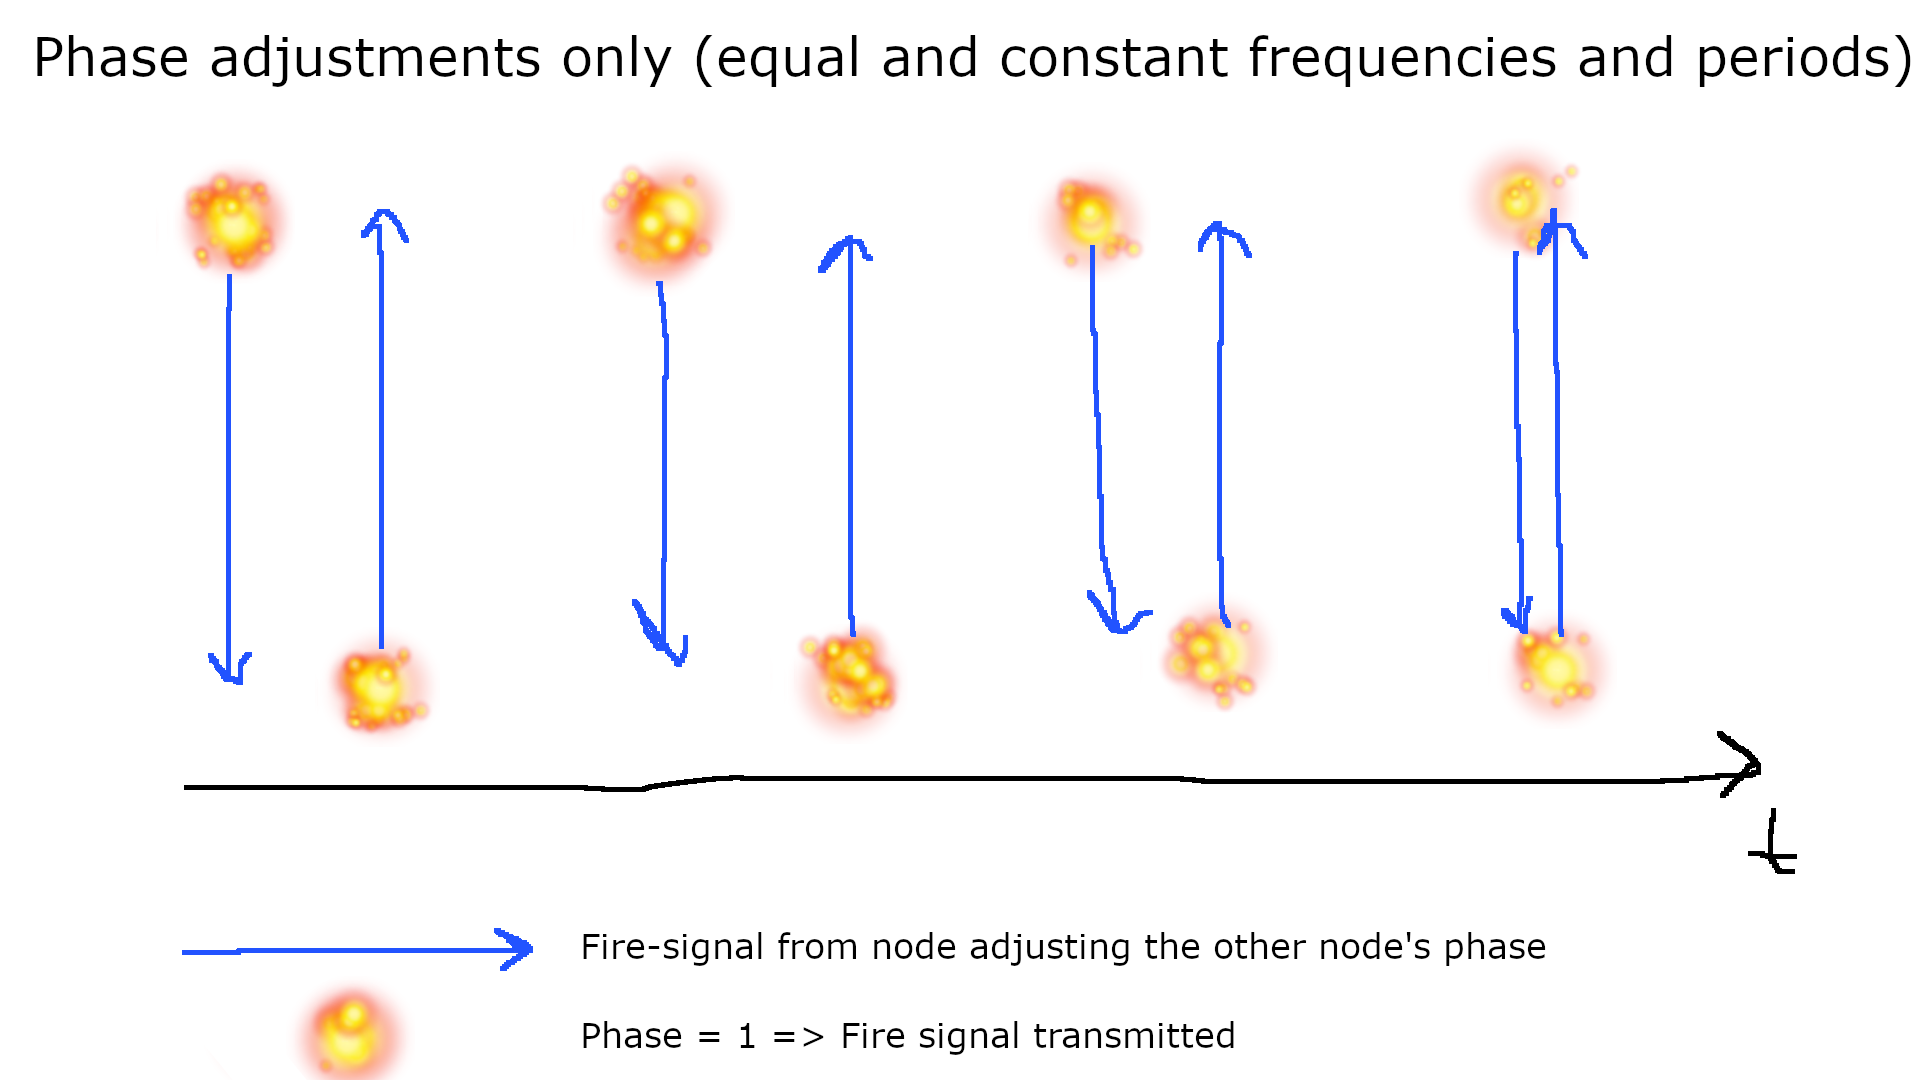
\includegraphics[width=0.90\textwidth]{Assets/Figures/phase_adjustments.png}
		\caption{Fase-justering (som om man skulle tappet med fingrene på et bord)}
	\end{figure}
}